\chapter{Estado da Arte} % (fold)
\label{cap:estado_da_arte}
\acresetall


No estado da arte quanto à representação de topologias de máquina encontra-se o projeto \textit{Hardware Locality} (hwloc) \cite{hwloc2010},
um pacote de \textit{software} amplamente utilizado que possui grande portabilidade.
Ele contém ferramentas de linha de comando, além de permitir que aplicações acessem as informações sobre a topologia por meio de uma API na linguagem C.

%\tratar{Servet - estima, LIKWID}
%
Entre os trabalhos relacionados ao tema,
há também o projeto LIKWID \cite{LIKWID},
um conjunto de utilidades para auxiliar no desenvolvimento de programas com foco no desempenho.
Suas funcionalidades são acessadas em parte por uma API, mas principalmente pela linha de comando.
É possível, entre outros, obter informações sobre a topologia das memórias \textit{cache} e utilizar contadores de \textit{hardware}.
%tem por objetivo melhorar o desempenho  a facilidade de uso
O LIWKID utiliza o hwloc, como pode ser visto no código fonte \cite{LIKWIDCod}.
%
Outro projeto com propósito semelhante é o Servet \cite{servet}, que obtém as informações utilizando \textit{benchmarks} para estimar as características da máquina.

O hwloc foi analisado neste trabalho devido ao seu uso em diversos projetos e,
em especial, no HieSchella \cite{HieSchella}, o qual poderia ter ganhos significativos de desempenho com os resultados deste trabalho.
As seções a seguir apresentam alguns aspectos relevantes do hwloc.



\section{Objetos}
\label{sec:objetos}

Objetos são uma abstração usada para representar todos os elementos presentes na topologia, tanto memória quanto núcleos.
A hierarquia de memória é modelada como uma árvore de objetos, onde cada nível contém objetos de apenas um tipo.
A topologia por completo é representada de forma mais detalhada por meio de várias ligações (ponteiros) entre objetos, conforme as suas relações na hierarquia.
Essas relações são definidas como:
\begin{itemize}
	\item Pai (\textit{parent}): nó pai na estrutura de árvore
	\item Filhos (\textit{children}): nós filhos na estrutura de árvore
	\item Irmãos (\textit{siblings}): nós com o mesmo pai
	\item Primos (\textit{cousins}): Objetos numa mesma profundidade (e, portanto, de mesmo tipo); todos os objetos que compõe um determinado nível (irmãos ou não) são primos
\end{itemize}
% TODO Criar macro
\begin{figure}[h]
	\caption{Relações entre objetos em topologias do hwloc. Fonte: \cite{hwlocImg}}
	\label{fig:relacoes}
	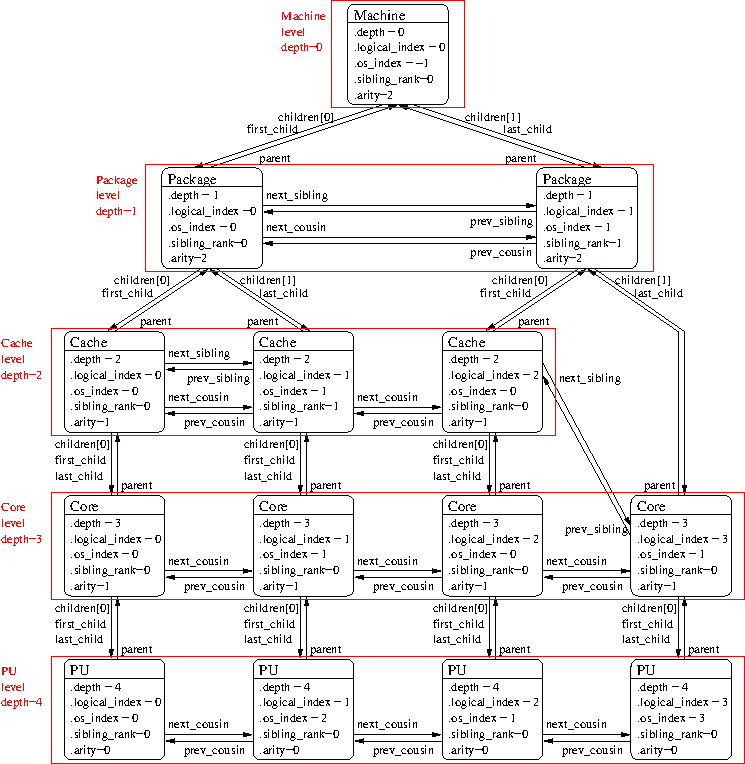
\includegraphics[width=\textwidth]{rec/img/relacoes}
\end{figure}
A Figura \ref{fig:relacoes} apresenta um exemplo dessas relações em uma dada topologia.
Ela ilustra, ainda, no ramo mais a direita, como hierarquias assimétricas (que possuem quantidades diferentes de objetos em ramos partindo do mesmo nó) são tratadas: podem surgir ``buracos'' devido a objetos de um mesmo tipo serem agrupados no mesmo nível.
% [Deixar mais claro] Buracos na hierarquia podem surgir porque o hwloc agrupa objetos do mesmo tipo no mesmo nível.
% Definir assimetria, segundo hwloc. Filhos com graus diferentes resulta em assimetria?
Portanto, objetos irmãos não estarão necessariamente no mesmo nível, e o conceito de profundidade não é exatamente o usado no contexto de estruturas de árvore, sendo possível irmãos terem profundidades diferentes.

Esse exemplo apenas ilustra o tratamento da assimetria.
Em casos reais, hierarquias assimétricas geralmente surgem devido ao acréscimo de objetos (chamados de grupos) na hierarquia para representar melhor a afinidade de dispositivos de entrada e saida,
deixando esses dispositivos mais próximos de algumas unidades de processamento do que das demais na árvore.

Essas relações acrescentadas à estrutura de árvore facilitam a navegação entre objetos, em troca do espaço adicional ocupado por cada ponteiro nos objetos.
Por exemplo, como indicado na figura, a partir de qualquer objeto, é possível navegar para o próximo primo (pelo ponteiro \texttt{next\_cousin}), ou para o próximo irmão (ponteiro \texttt{next\_sibling}), se existirem.
Além disso, todos os objetos são armazenados numa estrutura de arranjo de arranjos de objetos, semelhante a uma matriz, mas com arranjos internos de tamanho variável.
Cada um dos arranjos internos contém os objetos de um nível, e eles são organizados no arranjo externo na ordem dos níveis, de modo que é possível acessar o enésimo objeto de um dado nível diretamente usando essa estrutura.

%Figura X: https://www.open-mpi.org/projects/hwloc/doc/v1.11.2/diagram.png
Todos os objetos que compõe a hierarquia e outras estruturas de dados utilizadas na representação da topologia são armazenados em uma estrutura (\texttt{struct~hwloc\_topology}) que é utilizada pelas funções que acessam dados da topologia.


%?
\section{Funções e atributos}

Existem funções que podem ser utilizadas para acessar os objetos da hierarquia e informações sobre eles.
Entre elas, o hwloc possui diversas funções de percorrimento.
Estas permitem acessar nós da árvore que representa a hierarquia de forma absoluta ou relativa a outros nós.
Por exemplo, é possível encontrar o nó com um determinado índice dentro de um dado nível,
ou, a partir de algum nó, o próximo no mesmo nível.
Alguns exemplos de funções são:
\begin{itemize}
	\item \texttt{hwloc\_get\_nbobjs\_by\_type}: Informa quantos objetos de um determinado tipo existem, por exemplo, a quantidade de núcleos.
	\item \texttt{hwloc\_get\_cache\_covering\_cpuset}: Encontra a primeira memória \textit{cache} que abrange um dado conjunto de CPUs.
	\item \texttt{hwloc\_get\_ancestor\_obj\_by\_type}: Encontra o ancestral de um objeto que seja de um determinado tipo.
	\item \texttt{\texttt{hwloc\_get\_ancestor\_obj\_by\_depth}}: Semelhante à função anterior, procurando por nível em vez de tipo.
	\item \texttt{hwloc\_get\_common\_ancestor\_obj}: Encontra o ancestral comum mais próximo (ACMP) entre dois objetos, isto é, o nó de maior profundidade que é ancestral de ambos.
	%\item \texttt{}:
\end{itemize}

Essas funções foram analisadas quanto à complexidade com o objetivo de identificar pontos que poderiam ser melhorados do ponto de vista do desempenho.
Essa análise revelou que, em geral, elas têm tempo constante ($\bigO(1)$) ou linear na altura da árvore (\Oalt), que é o mesmo que $\bigO(\log N)$, onde $N$ é a quantidade de nós da árvore.
Além disso, foi analisado o projeto HieSchella, o qual possui código aberto e utiliza o hwloc \cite{HieSchella}.
Foram identificadas as chamadas mais importantes a funções do hwloc no HieSchella para se ter uma referência
de quais funções são mais relevantes para o desempenho dentro de um projeto real.
O Capítulo~\ref{cap:implementacao} apresenta o que foi feito em decorrimento dessas análises.

Os objetos ainda têm atributos que podem guardar diversas informações, como detalhes do sistema operacional ou da máquina, que podem ser coletadas automaticamente durante o descobrimento da topologia ou adicionadas manualmente.
Além disso, há várias informações específicas de \textit{caches}, como associatividade ou tamanho.
Também é possível associar estruturas arbitrárias aos objetos, conforme for necessário, usando dados de usuário (ponteiro \texttt{userdata}).


% >> Conjuntos de CPUs (cpusets)
\section{Conjuntos de CPUs}
\label{sec:conjuntos_de_cpus}

Cada objeto pode ter um \textit{cpuset} (conjunto de CPUs), que é um mapeamento dos núcleos existentes para \textit{bits} (\textit{bitmap}), usado para determinar quais núcleos estão sob o objeto na hierarquia, implementado como uma sequência de variáveis de 32 \textit{bits}, tantas quantas forem necessárias.
A implementação dos \textit{bitmaps} poderia ser otimizada para diminuir a quantidade de variáveis utilizadas em casos em que existam grandes quantidades de núcleos.
Algo nesse sentido é citado no respectivo arquivo fonte em um comentário sobre otimizações que poderiam ser realizadas \cite{hwlocCod}.